 
\documentclass[11pt,a4paper]{article}
\usepackage[utf8]{inputenc}		% LaTeX, comprend les accents !
\usepackage[T1]{fontenc}
\usepackage{natbib}	
%\usepackage[square,sort&compress,sectionbib]{natbib}		% Doit être chargé avant babel      
\usepackage[frenchb,english]{babel}
\usepackage{lmodern}
\usepackage{amsmath,amssymb, amsthm}
\usepackage{a4wide}
\usepackage[capposition=top]{floatrow}
\usepackage{verbatim}
\usepackage{float}
\usepackage{placeins}
\usepackage{flafter}
\usepackage{longtable}
\usepackage{import}
\usepackage{pdflscape}
\usepackage{rotating}
\usepackage{hhline}
\usepackage{multirow}
\usepackage{booktabs}
\usepackage[pdftex,pdfborder={0 0 0},colorlinks=true,linkcolor=blue,urlcolor=blue,citecolor=blue,bookmarksopen=true]{hyperref}
\usepackage{eurosym}
%\usepackage{breakcites}
\usepackage[autostyle]{csquotes}
%\usepackage{datetime}
\usepackage{natbib}
\usepackage{setspace}
\usepackage{lscape}
\usepackage[usenames]{color}
\usepackage{indentfirst}
\usepackage{forest}
\usepackage{url}
\usepackage{enumitem}
\usepackage{multirow}
\usepackage{subcaption}
\usepackage[justification=centering]{caption}
\bibliographystyle{agsm}

\usepackage{array}

\newcommand{\isEmbedded}{true}

\graphicspath{{../bordeaux/results/}}


\begin{document}

\selectlanguage{frenchb}
\title{Document préparatoire \\ Séance de travail des 5 et 6 octobre 2016}


\author{Sophie Cottet, Mahdi Ben Jelloul et Simon Rabat\'e}


\maketitle

% Introduction
Cette note propose des premières pistes d'estimation pour la modélisation de l'évolution des rémunérations à partir des grilles indiciaires dans les fonctions publiques territoriales et hospitalières. 
Dans un premier temps, nous revenons sur les processus que l'on souhaite modéliser. L'évolution de la rémunération des fonctionnaires dépend des changements de grades et des changements d'échelon au sein des grades. Nous cherchons ensuite à documenter ces processus dans les données transmises par la CDC. Le manque de profondeur temporel dans les données limite pour l'instant l'analyse des données. En conséquence, les suggestions de modélisation qui en découlent restent globalement spéculatives; les approches envisagées à ce stade sont toutefois décrites dans la troisième partie de ce document. Enfin, dans une dernière partie nous décrivons des méthodes de simulation à partir des estimations, pouvant servir de base aux tests d'adéquation des modèles économétriques voire à la simulations des trajectoires dans le modèle de microsimulation. 

% Section I: principe général 
\ifx\isEmbedded\undefined


\documentclass[11pt,a4paper]{article}
\usepackage[utf8]{inputenc}		% LaTeX, comprend les accents !
\usepackage[T1]{fontenc}
\usepackage{natbib}	
%\usepackage[square,sort&compress,sectionbib]{natbib}		% Doit être chargé avant babel      
\usepackage[frenchb,english]{babel}
\usepackage{lmodern}
\usepackage{amsmath,amssymb, amsthm}
\usepackage{a4wide}
\usepackage[capposition=top]{floatrow}
\usepackage{verbatim}
\usepackage{float}
\usepackage{placeins}
\usepackage{flafter}
\usepackage{longtable}
\usepackage{pdflscape}
\usepackage{rotating}
\usepackage{hhline}
\usepackage{multirow}
\usepackage{booktabs}
\usepackage[pdftex,pdfborder={0 0 0},colorlinks=true,linkcolor=blue,urlcolor=blue,citecolor=blue,bookmarksopen=true]{hyperref}
\usepackage{eurosym}
\usepackage{breakcites}
\usepackage[autostyle]{csquotes}
%\usepackage{datetime}
\usepackage{natbib}
\usepackage{setspace}
\usepackage{lscape}
\usepackage[usenames]{color}
\usepackage{indentfirst}

\usepackage{url}
\usepackage{enumitem}
\usepackage{multirow}
\usepackage{subcaption}
\usepackage[justification=centering]{caption}
\bibliographystyle{agsm}

\usepackage{array}

\begin{document}
\selectlanguage{frenchb}
\else \fi
%%%%%%%%%%%%%%%%%%%%%%%%%%%%%%%%%%%%%%%%%%%%%%%%%%%%%%%%%%%%%%%%%%%%%%%%%%%%%%%%%%%%%%%%%%%%%%%%%%%%%%%%%%%%%%



\section{L'objectif: modéliser les rémunérations à partir des grilles}


\subsection*{Retour sur la classification des emplois}

L'organisation de la carrière d'un fonctionnaire est fondée sur une grille de classement des emplois, avec différents niveaux:
 
\begin{enumerate}[leftmargin=1cm ,parsep=0cm,itemsep=0cm,topsep=0cm] 
\item Les cadres ou corps d'emploi,
\item Les filières: regroupements informels des corps d'emploi (10 dans la FPT, 6 dans la FPH), 
\item Les catégories hiérarchiques: les fonctionnaires peuvent être de catégorie A, B ou C,
\item Les grades: chaque corps d'emploi est segmenté en un ou plusieurs grades, régulés par un statut particulier,
\item Les échelons définissant le niveau de l'indice brut au sein du grade. 
\end{enumerate}

% TODO: j'inverserai les 3 premiers pour les mettre dans l'ordre 2
% Modélisation corps/grade/échelon

\vspace{0.5cm}

La grille de rémunération est définie pour chaque grade: elle donne le niveau de l'indice brut pour un échelon donné. 


Points à préciser: 
\begin{itemize}[leftmargin=1cm ,parsep=0cm,itemsep=0cm,topsep=0cm] 
%\item Y a-t-il bien une délimitation nette entre cadres/filières et catégories hiérarchiques? (la filière X n'est composée que de fonctionnaires de catégorie A). 
\item Quelles conditions de passage d'un grade à l'autre au sein d'un corps ? Passage automatique comme pour les échelons ou plus discrétionnaire ? %Question à supprimer, cf. mail Sophie
\item Dans quelle mesure la carrière au sein d'un corps est linéaire (grade 1 -> grade 2 -> grade 3 vs. grade 1 -> grade 2 ou 3)? 

\item A quoi correspond la durée 
 moyenne dans un échelon ? Est-ce empirique ? Si elle a un valeur législative, comment cette durée est-elle opérante ?
\end{itemize}


\subsection*{Les phénomènes à modéliser}

Si on met de côté pour l'instant le taux de prime, la modélisation du salaire des fonctionnaires dépend de l'évolution de la rémunération, elle-même définie directement par l'évolution de l'indice brut. 

Modéliser l'évolution de l'indice revient donc à modéliser deux phénomènes principaux de la carrière d'un individu: 
\begin{itemize}[leftmargin=1cm ,parsep=0cm,itemsep=0cm,topsep=0cm] 
\item La progression au sein d'un grade, c'est-à-dire la vitesse à laquelle les échelons sont franchis,
\item Les changements de grade, qui regroupent en fait deux phénomènes potentiellement très différents: 
	\begin{itemize}[leftmargin=1cm ,parsep=0cm,itemsep=0cm,topsep=0cm] 
	\item Les changements de grades en fin de grille
	\item Les changements de grades avant la fin de la grille
	\end{itemize}
\end{itemize} 

\vspace{0.2cm}

La question centrale de la modélisation de l'évolution est donc la suivante: pour quel type de phénomène a-t-on de la variabilité inter-individuelle? Plus les grilles sont rigides, plus la modélisation choisie peut-être simple. A l'extrême, si la durée dans chaque échelon est fixe et que le changement de grade suit une règle fixe (par exemple, "tous les individus arrivés au bout du grade G1 passent au grade G2"), l'évolution de la rémunération dépend directement de l'évolution des grilles et ne nécessite pas de travail de modélisation. La modélisation est nécessaire car, en réalité, la carrière des individus ne suit pas un chemin prédéfini. L'enjeu principal est donc la modélisation de la déviation par rapport à ce "tapis roulant". Cette déviation peut intervenir au niveau de la durée passée dans chaque échelon, au niveau du moment où intervient le changement de grade (avant la fin de la grille ou en fin de grille), et au niveau du grade de destination après le changement. 

Il s'agit d'une question en partie législative: dans quelle mesure est fixe la durée passée dans l'échelon (durée minimale, durée maximale, ou durée fixe), et dans quelle mesure le passage d'un grade à l'autre est automatique au sein d'un corps (Quels sont les conditions de promotions: concours, ou simplement âge ou durée dans le grade ?). A rigidité législative donnée, il s'agit d'une question empirique:
\begin{itemize}
    \item Quelle variance observe-t-on dans la durée passée dans chaque échelon au sein d'un grade ? Quelle proportion d'individus est promue au sein de son corps dans le grade supérieur ?
   \item A quel moment ces promotions se produisent-elles ? 
   \item Quelle proportion d'individu change de grade sans passer dans le grade immédiatement supérieur (changement de corps, de catégorie, de fonction publique) ?
\end{itemize}  


\subsection*{Une première tentative de schématisation}

Le schéma implicite que nous avons en tête, et qui doit être confronté aux données, est le suivant: les individus suivent globalement l'évolution dans leur corps de rattachement, avec des passages d'un échelon à l'autre et d'un grade à l'autre. L'évolution n'est pas totalement déterministe: la vitesse d'évolution dans la grille du corps peut varier, certains individus peuvent ne pas satisfaire les critères de passage de grade, et pour certains grades il peut y avoir plusieurs trajectoires possibles à l'intérieur du corps. A côté de cette évolution globalement linéaire, il peut y avoir également des changements de grade qui ne suivent pas directement la trajectoire dans le corps, avec des changements de corps ou de catégorie par concours. Ces types de mouvement peuvent être concentrés sur des individus spécifiques (les \textit{movers}, par opposition aux \textit{stayers} qui suivent la grille), ou répartis de manière globalement aléatoire entre les individus. 

La frontière entre les changements de grade \og normaux \fg{}  et les changement de grade plus importants n'est pas forcément très nette pour l'instant: si un individu change de grade de manière précoce par un concours qui lui permet d'accéder au grade immédiatement supérieur, doit-on considérer cela comme un saut de grille ou comme une progression rapide dans le corps? Notre position \textit{a priori} est que, dans le cas général, le changement de grade au sein du corps se fait quand l'ensemble du grade courant a été parcouru. Si en pratique, les changements interviennent à tout moment, la distinction envisagée n'est pas forcément pertinente.


Dans la partie suivante, nous tentons de documenter ces questions à partir des données disponibles à ce stade. 


\vspace{0.5cm}
Points à préciser: 
\begin{itemize}[leftmargin=1cm ,parsep=0cm,itemsep=0cm,topsep=0cm] 
    \item Quelle interaction entre le module \og rémunération \fg\ et les modules \og carrière \fg\ et \og affiliation \fg ?   
    \item[] Par exemple, doit-on traiter différemment un mouvement de la FPT vers la FPE et un changement important de corps au sein de la FPE? 
% Comment différencier un changement de grade d'une sortie de la FP ou d'une disponibilité, sachant que ces deux phénomènes ne sont pas forcément décorrélés (un individus peut démissionner plus facilement de la FPT-FPH s'il ne peut pas accéder à un grade supérieur) ? 
\end{itemize}


%%%%%%%%%%%%%%%%%%%%%%%%%%%%%%%%%%%%%%%%%%%%%%%%%%%%%%%%%%%%%%%%%%%%%%%%%%%%

\ifx\isEmbedded\undefined
\newpage
\bibliographystyle{../../Divers/myagsm} 
\bibliography{../../Divers/biblio_these}
\end{document}
\else \fi




% Section II: data
\ifx\isEmbedded\undefined


\documentclass[11pt,a4paper]{article}
\usepackage[utf8]{inputenc}		% LaTeX, comprend les accents !
\usepackage[T1]{fontenc}
\usepackage{natbib}	
%\usepackage[square,sort&compress,sectionbib]{natbib}		% Doit être chargé avant babel      
\usepackage[frenchb,english]{babel}
\usepackage{lmodern}
\usepackage{amsmath,amssymb, amsthm}
\usepackage{a4wide}
\usepackage[capposition=top]{floatrow}
\usepackage{verbatim}
\usepackage{float}
\usepackage{placeins}
\usepackage{flafter}
\usepackage{longtable}
\usepackage{pdflscape}
\usepackage{rotating}
\usepackage{hhline}
\usepackage{multirow}
\usepackage{booktabs}
\usepackage[pdftex,pdfborder={0 0 0},colorlinks=true,linkcolor=blue,urlcolor=blue,citecolor=blue,bookmarksopen=true]{hyperref}
\usepackage{eurosym}
\usepackage{breakcites}
\usepackage[autostyle]{csquotes}
%\usepackage{datetime}
\usepackage{natbib}
\usepackage{setspace}
\usepackage{lscape}
\usepackage[usenames]{color}
\usepackage{indentfirst}

\usepackage{url}
\usepackage{enumitem}
\usepackage{multirow}
\usepackage{subcaption}
\usepackage[justification=centering]{caption}
\bibliographystyle{agsm}

\usepackage{array}



\graphicspath{{../../bordeaux/results/}}


\begin{document}



\else \fi
%%%%%%%%%%%%%%%%%%%%%%%%%%%%%%%%%%%%%%%%%%%%%%%%%%%%%%%%%%%%%%%%%%%%%%%%%%%%%%%%%%%%%%%%%%%%%%%%%%%%%%%%%%%%%%



\section{L'analyse des données: résultats préliminaires}

En amont du choix de modélisation, il est nécessaire de documenter la variabilité individuelle dans les différents phénomènes que l'on souhaite modéliser. Par rapport à des trajectoires totalement déterministes, l'aléa peut venir (i) de la durée passée dans l'échelon (ii) de la possibilité de changement de grade en milieu de grille et (iii) du choix du changement de grade en fin de grille. 

\subsection{Les données disponibles à ce stade}

TODO

\subsection{Vitesse et typologie des changements de grade: besoin de recul temporel}

Documenter les différents phénomènes de manière précise suppose de pouvoir retracer la trajectoire individuelle complète, avec ses changements de grades et d'échelon sur une durée assez longue. La profondeur temporelle est nécessaire pour pouvoir dire combien de temps un individu donné reste dans son échelon (vitesse, phénomène 1) et pour savoir si l'individu change de grade en milieu de grille (phénomène 2) ou en fin de grille (phénomène 3). 

A ce stade il y a donc un travail de complétion à faire, sur la base de la note transmise par P. Joubert, pour retracer l'évolution du couple (grade, échelon) sur une période plus longue que les 4 ans (2011-2015) actuellement disponibles. 

Une fois ces trajectoires reconstituées, nous chercherons à savoir: 
\begin{itemize}[leftmargin=1cm ,parsep=0cm,itemsep=0cm,topsep=0cm] 
\item La dispersion de la durée passée dans les échelons, à la fois entre individus d'un même grade et entre les différents grades. 
\item A quel moment interviennent les changements de grade? Dans quelle mesure les changements de grade avant la fin de la grille sont (i) fréquents (ii) différents des changements de grade en fin de grilles. 
\end{itemize}



\subsection{Analyser les grades de destination: premiers résultats}

L'analyse des données sur les années 2011-2014 permet de documenter une autre question importante par rapport aux choix de modélisation: le grade de destination quand on observe un changement de grade pour un individu donné. A ce stade nous n'avons pas localisé le changement de grade sur la grille. L'approche adoptée est la suivante: pour chaque grade, nous considérons les années pour laquelle nous observons un changement de grade entre l'année $n$ et l'année $n+1$, et calculons les outputs suivants: 


\begin{itemize}[leftmargin=1cm ,parsep=0cm,itemsep=0cm,topsep=0cm] 
\item Le nombre de grades possibles en $n+1$
\item La proportion d'individus passant dans le grade le plus représenté en $n+1$, les deux plus représentés, les trois plus représentés, et les 5 plus représentés. 
\end{itemize}

Les moyennes sur l'ensemble de la population, pondérée ou non en fonction du nombre de transitions observées pour le grade considérée, sont présentées à la table \ref{means}. Même s'il existe un nombre élevé de transitions possibles en moyenne, la grande majorité des transitions se fait vers un petit nombres de grade possible. Ainsi par exemple 94\% des transitions observés se font vers les 3 destinations principales (propres à chaque grade). Ce constat est confirmé au graphique \ref{pct},

\begin{table}[ht]
\label{means}
\centering
\caption{Destinations en cas de changement de grade} 
\begin{tabular}{l|cc}
  \hline
 & Moyenne simple & Moyenne pondérée \\ 
  \hline
Nombre de destinations & 11.4 & 45.5 \\ 
  \% pour la destination majoritaire & 66.1 & 58.8 \\ 
  \% pour les 2 destinations majoritaires & 87.4 & 87.0 \\ 
  \% pour les 3 destinations majoritaires & 93.6 & 92.8 \\ 
  \% pour les 5 destinations majoritaires & 97.5 & 96.1 \\ 
   \hline
\end{tabular}
\end{table}



\begin{figure}[t]
  \label{pct}
\caption{Distribution de la proportion de transitions vers les destinations principales}
\vspace{-0.1cm}
\centering
 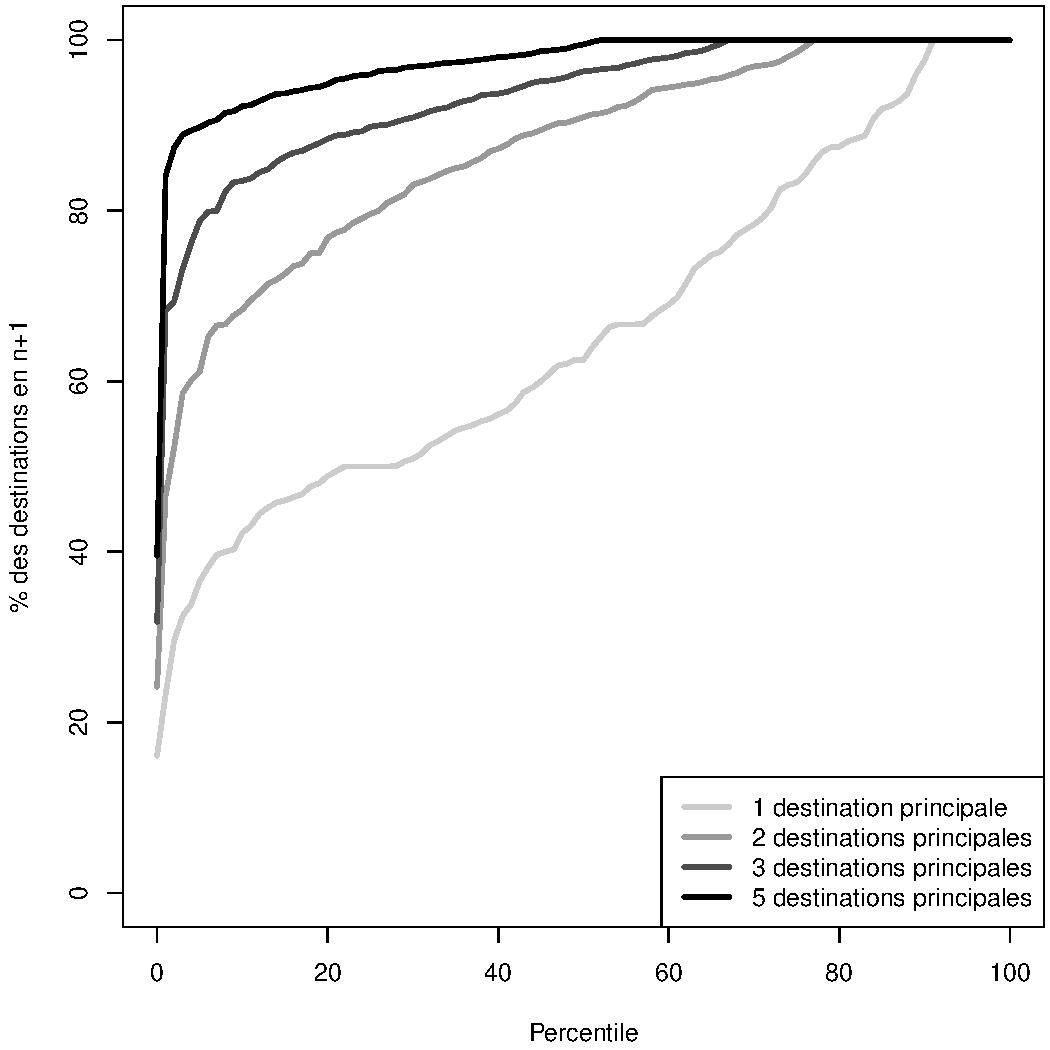
\includegraphics[width=0.7\linewidth]{pct.pdf}
\vspace{0.1cm}  
\begin{minipage}{12cm}%
\small \textsc{Lecture:} Pour environ 50 \% des grades, les 5 destinations les plus fréquentes représentent 100 \% des transitions observées.  
 \end{minipage}%
\end{figure}


Questions à discuter
\begin{enumerate}[leftmargin=1cm ,parsep=0cm,itemsep=0cm,topsep=0cm] 
\item Quel statut des transitions vers une missing value? Problème de donnée ou disponibilité ou sortie de la FP? Module rémunération, carrière ou affiliation? 
\end{enumerate}



%%%%%%%%%%%%%%%%%%%%%%%%%%%%%%%%%%%%%%%%%%%%%%%%%%%%%%%%%%%%%%%%%%%%%%%%%%%%

\ifx\isEmbedded\undefined
\newpage
\bibliographystyle{../../Divers/myagsm} 
\bibliography{../../Divers/biblio_these}
\end{document}
\else \fi





% Section III: Modélisation
\ifx\isEmbedded\undefined


\documentclass[11pt,a4paper]{article}
\usepackage[utf8]{inputenc}		% LaTeX, comprend les accents !
\usepackage[T1]{fontenc}
\usepackage{natbib}	
%\usepackage[square,sort&compress,sectionbib]{natbib}		% Doit être chargé avant babel      
\usepackage[frenchb,english]{babel}
\usepackage{lmodern}
\usepackage{amsmath,amssymb, amsthm}
\usepackage{a4wide}
\usepackage[capposition=top]{floatrow}
\usepackage{verbatim}
\usepackage{float}
\usepackage{placeins}
\usepackage{flafter}
\usepackage{longtable}
\usepackage{pdflscape}
\usepackage{rotating}
\usepackage{hhline}
\usepackage{multirow}
\usepackage{booktabs}
\usepackage[pdftex,pdfborder={0 0 0},colorlinks=true,linkcolor=blue,urlcolor=blue,citecolor=blue,bookmarksopen=true]{hyperref}
\usepackage{eurosym}
\usepackage{breakcites}
\usepackage[autostyle]{csquotes}
%\usepackage{datetime}
\usepackage{natbib}
\usepackage{setspace}
\usepackage{lscape}
\usepackage[usenames]{color}
\usepackage{indentfirst}

\usepackage{forest}
\usepackage{url}
\usepackage{enumitem}
\usepackage{multirow}
\usepackage{subcaption}
\usepackage[justification=centering]{caption}
\bibliographystyle{agsm}

\usepackage{array}

\begin{document}

\else \fi
%%%%%%%%%%%%%%%%%%%%%%%%%%%%%%%%%%%%%%%%%%%%%%%%%%%%%%%%%%%%%%%%%%%%%%%%%%%%%%%%%%%%%%%%%%%%%%%%%%%%%%%%%%%%%%



\section{Les modélisations économétriques envisagées}

Comme précisé précédemment, trois processus distincts doivent être modélisés: 
\begin{enumerate}[leftmargin=1cm ,parsep=0cm,itemsep=0cm,topsep=0cm]
\item La vitesse de franchissement des échelons au sein d'un grade
\item Le passage au grade supérieur dans le corps (\textit{a priori}, quand l'individu arrive en fin de grille)
\item Les mouvements plus importants: changement de corps, de catégorie hiérarchique, de FP (\textit{a priori}, pouvant intervenir n'important quand)
\end{enumerate}

Dans cette section nous mentionnons les pistes envisagées pour la modélisation de ces différents processus. Il s'agit de pistes de réflexions engagées avant une étude approfondie des données, et ne sont donc pas définitives. 


\subsection{Modéliser la vitesse dans le grade avec des effets fixes?}

Par vitesse dans le grade nous entendons la durée passée dans les échelon successifs d'un grade donné. Nous n'avons pas d'idée \textit{a priori} sur l'ampleur du phénomène. La dimension législative est sans doute importante: la progression dans l'échelon est parfois contrainte par une durée minimale et une durée maximale, voire une durée fixe pour certains grades. 

Un première question sera donc de savoir si cette dimension doit être modélisée (dans quelle mesure observe-t-on de la dispersion interindividuelle sur ce point?), et comment peut-on prendre en compte les législations spécifiques à chaque grade. 

La modélisation envisagée est la suivante: chaque individu possède une vitesse relative propre (un effet fixe), qui détermine la durée passée dans l'échelon relativement aux autre individus du grade. L'approche par effets fixes se justifient car, \textit{a priori}, la modélisation de la vitesse dans l'échelon est nécessaire uniquement si ce sont les mêmes individus qui franchissent plus rapidement les échelons au cours de leur carrière. L'idée est donc d'identifier des individus plus ou moins \og rapides \fg{} dans leur progression. Ces effets fixes se rapprochent des effets fixes dans les équations de salaires usuellement utilisées dans les modèles de microsimulation.  
A chaque date $t$, l'individu franchit ou non l'échelon en fonction de (i) sa durée passée dans l'échelon (ii) la durée \og normale \fg{} dans l'échelon et (iii) sa vitesse relative de franchissement des échelons. 

Certains tests rapides pourront être mis en \oe uvre pour attester de la pertinence d'une telle approche. Une fois reconstituée une trajectoire professionnelle de long terme, nous pourrons vérifier que les individus qui franchissent relativement plus rapidement un échelon donné, le font également sur l'ensemble de la grille considérée d'une part, et sur les autres grilles sur lesquelles on l'observe d'autre part. L'idée étant de vérifier que l'on peut modéliser la vitesse relative par un terme fixe au cours de la carrière. 


\subsection{Modéliser le \og choix \fg{} en fin de grille par un modèle de choix discret?}

Quand l'individu arrive en fin de grille (par hypothèse, ce qui peut se discuter\footnote{Étant donné que l'on observe des chevauchement dans les indices bruts des grilles d'un même corps, nous pouvons envisager que la décision du changement de grille peut intervenir avant l'arrivée au dernier échelon. Le choix du moment où l'on modélise la décision du passage au grade supérieur est conditionné par l'analyse de la temporalité des changement de grade, devant être menée en amont. }), il peut faire face à différents \og choix \fg{}: (i) passer dans le (ou les) grades supérieurs dans leur corps, (ii) rester à l'échelon maximal du grade ou (iii) quitter le corps, voire la fonction publique. 

Cette problématique suggère une modélisation du phénomène comme \og choix discrets \fg\ : il s'agirait d'estimer la probabilité d'un ensemble de choix, non ordonnés.
C'est une modélisation répandue notamment en économie du travail, lorsqu'on cherche à estimer la probabilité d'être en emploi à temps plein, en emploi à temps partiel,
en recherche d'emploi, actif inoccupé, \textit{etc.} L'estimation se fait par logit multinomial.



\paragraph{L'hypothèse d'indépendance des hypothèses non pertinentes}\footnote{\textit{IIA: Independance from Irrelevant alternatives}} Une limite importante de ce type de modélisation est que, le logit multinomial étant une généralisation du modèle binaire, on suppose que le choix entre deux alternatives est indépendant des autres alternatives. Plus précisément, la probabilité de choisir une alternative par rapport à une deuxième n'est pas conditionné par le contenu d'une troisième alternative. 

L'exemple classique est le choix d'un mode de transport, entre le vélo, le bus et la voiture. La probabilité de choisir la voiture plutôt que le vélo n'est pas indépendante de la qualité du service de bus: une amélioration de la qualité conduit à augmenter la probabilité de choisir le vélo par rapport à la probabilité de choisir la voiture, car la première n'est \textit{a priori} pas affecté par la qualité du bus mais la deuxième l'est. Une solution usuelle est d'utiliser des logits emboités, regroupant les choix potentiellement corrélés. On décomposera le choix vélo, voiture et bus en un choix entre vélo et véhicule motorisé, choix lui même décomposé entre un choix entre voiture et bus. 

%Cette hypothèse ne semble pas problématique dans le cas de l'exemple donné, mais si on souhaite aussi modéliser le congé maladie, la mise en disponibilité ou le détachement, l'hypothèse est moins crédible.

Comment cela se transpose-t-il au cas étudié? Supposons qu'il y a 4 alternatives possibles pour un individu se trouvant au dernier échelon du grade 1 d'une fonction publique donnée: (i) aller dans le grade 2, (ii) aller dans le grade 3, (iii) rester dans le grade 1, et (iv) quitter la fonction publique (ou changer de fonction publique). \textit{A priori}, l'hypothèse IIA n'est pas respectée pour les alternatives (i) et (iii). Si le grade 3 devient relativement moins attractif, on peut supposer que la probabilité de (iv) n'est pas affectée alors que la probabilité de (i) pourrait l'être car le contenu du grade 1 est sans doute plus proche du contenu du grade 2. Une première étape évidente serait donc d'utiliser un logit emboîté rassemblant les différents  grades potentiels au sein de la FP dans lequel l'individu se trouve. Nous nous ramenons donc à trois issues potentielles (i) être promu au sein de la FP considérée, (ii) ne pas être promus et rester (iii) ne pas être promu et quitter le grade, le (i) pouvant être redécomposé en différents grades possibles. 
L'hypothèse IIA est-elle vérifiée dans ce cas ? Dans le choix entre (i) et (ii), une modification des perspectives extérieures à la FP considérée (par exemple un concours de changement de FP) devrait plus affecter les individus qui seraient restés dans le grade que les individus qui sont promus quoiqu'il arrive. Il semble donc également pertinent de regrouper les alternatives (ii) et (iii) dans le cadre d'un logit emboité. 

Nous sommes donc ramenés à un double logit emboité. 



\tikzset{
Above/.style={
  midway,
  above,
  font=\scriptsize,
  text width=1.5cm,
  align=center,
  },
Below/.style={
  midway,
  below,
  font=\scriptsize,
  text width=1.5cm,
  align=center
  }
}

\begin{center}
\begin{forest} 
for tree={
  grow=east,
  draw=cyan,
  circle,
  line width=0.2pt,
  parent anchor=east,
  child anchor=west,
  edge={draw=cyan},
  edge label={\Huge\color{black}},
  edge path={
    \noexpand\path[\forestoption{edge}]
      (!u.parent anchor) -- ([xshift=-2cm].child anchor) --    
      (.child anchor)\forestoption{edge label};
  },
  l sep=2cm,
} 
[,rectangle, s sep=35pt,
  [,edge label={node[Below]{Pas de promotion}}
    [,edge label={node[Below]{Quitter la FP considérée}}
    ]
    [,edge label={node[Above]{Rester dans grade 1}}
    ]
  ]
  [,edge label={node[Above]{Promotion dans la FP considérée}}
    [,edge label={node[Below]{Grade 3}}
    ]
    [,edge label={node[Above]{Grade 2}}
    ]
  ]
]
\end{forest}

\end{center}

\vspace{0.5cm}

Une autre possibilité serait de modéliser les sorties du corps en fin de grille de manière séparée, avec les changements de grade en cours de grille, évoqués ci-dessous. La modélisation représentée ci-dessus revient à faire l'hypothèse implicite que les changement de corps en fin de grille sont davantage liés à un manque de perspective dans le corps (individus bloqués en fin de grille), alors que les changement de corps en cours de grille sont plus \og positifs \fg{}. Mais il s'agit à ce stade de pure spéculation. Nous pourrons tester dans une certaine mesure cette hypothèse quand nous pourrons comparer les types de changement de grades en fin de grille et sur l'ensemble de la grille. 


\subsection{Modéliser les changement de grade en cours de grille: modèle de durée, choix discret, ou tirage aléatoire?}

A tout moment, les fonctionnaires peuvent changer de statut (de grade, de catégorie, de corps), par exemple en passant un concours. Nous considérons à part ce type de mouvement, en les considérant comme une déviation par rapport au parcours défini par l'évolution \og naturelle \fg{}  au sein des grades et des corps. 

Ce type de processus est potentiellement complexe à modéliser, car les destinations possible quand un individu quitte son grade sont nombreuses: changement de grade au sein d'un corps, changement de catégorie, changement de fonction publique, sortie de la fonction publique. C'est d'ailleurs sur ce type de processus que les interactions avec les modules affiliations et carrières sont les plus difficiles à gérer. 

La complexité de la modélisation doit être comparée à l'importance du phénomène: si le processus représente une part faible des évolutions observées, une modélisation relativement sommaire est envisageable. Ainsi par exemple à chaque pas temporelle une certaines proportion d'individus peut être tirés puis envoyé vers un grade différent (avec pour seule contrainte un indice brut supérieur). Cette modélisation peut-être affiné dans le cadre d'un modèle binaire (logit ou probit) faisant dépendre la probabilité de changer de grade de certaines caractéristiques observables. 

Si ce processus est plus important qu'envisagé \textit{a priori}, une modélisation plus fine devra être adoptée. Deux grands type d'approche sont considérés à ce stade. Premièrement, des modèles à choix discret peuvent être testés A chaque date, un fonctionnaire fait face à un ensemble de choix: rester sur son \og tapis roulant \fg{}, passer un concours, partir dans le privé, etc. Un tel modèle peut en théorie être estimé sur les données passées, éventuellement après regroupement des alternatives proches. Nous envisageons également un modèle de durée, avec différents états concurrents, modélisant la survie dans le grade. A chaque date, l'individu a une probabilité de quitter le grade dans lequel il est, selon certaines caractéristiques observables (niveau dans le grade), et éventuellement inobservables en prenant en compte les durées passées observée dans les grades ou échelons précédents (\textit{multispell duration models}). 


\bigskip

L'analyse de la temporalité des changements de grade est donc un préalable indispensable à la poursuite de la réflexion sur la modélisation de la rémunération. Les modélisations proposées reposent sur des représentations \textit{a priori} des trajectoires indiciaires qui doivent être confrontées aux données. En particulier, notre analyse est structurée autour de la distinction entre les changements de grade \og naturels \fg{} (en fin de grille, au sein du corps, vers les grades supérieurs normaux) et plus imprévisibles (à tout moment et a priori plus importants: changement de corps, de catégorie, de fonction publique).  

Les questions à traiter en priorité sont les suivantes: 
\begin{itemize}
    \item Comment les changements de grades sont-ils repartis dans la grille? Sont-ils concentrés sur les derniers échelons ?
    \item Les changements de fin d'échelon sont-ils bien plus prévisibles que les autres changements observés ?     
\end{itemize}

Des réponses à ces questions dépendent la pertinence des choix de modélisations envisagés.

%%%%%%%%%%%%%%%%%%%%%%%%%%%%%%%%%%%%%%%%%%%%%%%%%%%%%%%%%%%%%%%%%%%%%%%%%%%%

\ifx\isEmbedded\undefined
\newpage
\bibliographystyle{../../Divers/myagsm} 
\bibliography{../../Divers/biblio_these}
\end{document}
\else \fi





% Section IV: Simulation
\ifx\isEmbedded\undefined


\documentclass[11pt,a4paper]{article}
\usepackage[utf8]{inputenc}		% LaTeX, comprend les accents !
\usepackage[T1]{fontenc}
\usepackage{natbib}	
%\usepackage[square,sort&compress,sectionbib]{natbib}		% Doit être chargé avant babel      
\usepackage[frenchb,english]{babel}
\usepackage{lmodern}
\usepackage{amsmath,amssymb, amsthm}
\usepackage{a4wide}
\usepackage[capposition=top]{floatrow}
\usepackage{verbatim}
\usepackage{float}
\usepackage{placeins}
\usepackage{flafter}
\usepackage{longtable}
\usepackage{pdflscape}
\usepackage{rotating}
\usepackage{hhline}
\usepackage{multirow}
\usepackage{booktabs}
\usepackage[pdftex,pdfborder={0 0 0},colorlinks=true,linkcolor=blue,urlcolor=blue,citecolor=blue,bookmarksopen=true]{hyperref}
\usepackage{eurosym}
\usepackage{breakcites}
\usepackage[autostyle]{csquotes}
%\usepackage{datetime}
\usepackage{natbib}
\usepackage{setspace}
\usepackage{lscape}
\usepackage[usenames]{color}
\usepackage{indentfirst}

\usepackage{url}
\usepackage{enumitem}
\usepackage{multirow}
\usepackage{subcaption}
\usepackage[justification=centering]{caption}
\bibliographystyle{agsm}

\usepackage{array}

\begin{document}

\else \fi
%%%%%%%%%%%%%%%%%%%%%%%%%%%%%%%%%%%%%%%%%%%%%%%%%%%%%%%%%%%%%%%%%%%%%%%%%%%%%%%%%%%%%%%%%%%%%%%%%%%%%%%%%%%%%%



\section{Microsimulation}


Afin de valider la performance modélisation retenue et les résultats de l'estimation économétrique, il nous semble utile de pouvoir réaliser une simulation rétrospective. En partant d'un état initial plus ou moins ancien et en faisant évoluer individuellement les agents, nous espérons être en mesure de détecter les limites des différentes modélisations pour les améliorer itérativement. A cette fin, il nous faut pouvoir microsimuler de façon efficace (temps de calcul, gestion de la mémoire) l'évolution de la population initiale.  


\subsection{Le parcours dans le grade}

Nous avons réalisé un prototype de parcours dans le grade à une vitesse de passage d'échelon donnée tout en respectant la législation et notamment les changements de grilles au cours du temps. Nous avons tenté de vectoriser au maximum le programme pour que l'exécution soit la plus rapide possible.
Les boucles se font donc sur les grades représentés et si nécessaires les échelons représentés. L'algorithme consiste à appliquer successivement les opérations suivantes:
\begin{itemize}
	\item Renseigner l'état initial des individus (date de l'observation, grade, échelon)
	\item Déterminer la date d'effet de la grille en cours et de la suivante
	\item Calcul de la durée dans l'échelon selon la grille en effet à l'état initial (et la vitesse de parcours de l'échelon le cas échéant)
	\item Calcul de la date d'effet d'une éventuelle grille réformée avant la fin de l'échelon
	\item Calcul de la durée dans l'échelon avec cette nouvelle grille
	\item Calcul de la durée effective dans l'échelon
	\item Calcul de la date de fin dans l'échelon
\end{itemize}
 

\subsection{Les changements de grade}

Si le modèle économétrique permets d'identifier les dates de changements de grade en cours de grade ou les modalités de promotion au grade supérieur, il devrait être possible de le coupler à l'algorithme précédent pour obtenir un algorithme permettant de simuler une carrière complète.





%%%%%%%%%%%%%%%%%%%%%%%%%%%%%%%%%%%%%%%%%%%%%%%%%%%%%%%%%%%%%%%%%%%%%%%%%%%%

\ifx\isEmbedded\undefined
\newpage
\bibliographystyle{../../Divers/myagsm} 
\bibliography{../../Divers/biblio_these}
\end{document}
\else \fi



\end{document}


